\documentclass[journal,12pt,twocolumn]{IEEEtran}

\usepackage{setspace}
\usepackage{gensymb}

\singlespacing


\usepackage[cmex10]{amsmath}

\usepackage{amsthm}

\usepackage{mathrsfs}
\usepackage{txfonts}
\usepackage{stfloats}
\usepackage{bm}
\usepackage{cite}
\usepackage{cases}
\usepackage{subfig}

\usepackage{longtable}
\usepackage{multirow}

\usepackage{enumitem}
\usepackage{mathtools}
\usepackage{steinmetz}
\usepackage{tikz}
\usepackage{circuitikz}
\usepackage{verbatim}
\usepackage{tfrupee}
\usepackage[breaklinks=true]{hyperref}
\usepackage{graphicx}
\usepackage{tkz-euclide}
\usepackage{float}

\usetikzlibrary{calc,math}
\usepackage{listings}
    \usepackage{color}                                            %%
    \usepackage{array}                                            %%
    \usepackage{longtable}                                        %%
    \usepackage{calc}                                             %%
    \usepackage{multirow}                                         %%
    \usepackage{hhline}                                           %%
    \usepackage{ifthen}                                           %%
    \usepackage{lscape}     
\usepackage{multicol}
\usepackage{chngcntr}

\DeclareMathOperator*{\Res}{Res}

\renewcommand\thesection{\arabic{section}}
\renewcommand\thesubsection{\thesection.\arabic{subsection}}
\renewcommand\thesubsubsection{\thesubsection.\arabic{subsubsection}}

\renewcommand\thesectiondis{\arabic{section}}
\renewcommand\thesubsectiondis{\thesectiondis.\arabic{subsection}}
\renewcommand\thesubsubsectiondis{\thesubsectiondis.\arabic{subsubsection}}


\hyphenation{op-tical net-works semi-conduc-tor}
\def\inputGnumericTable{}                                 %%

\lstset{
%language=C,
frame=single, 
breaklines=true,
columns=fullflexible
}
\begin{document}
\newtheorem{theorem}{Theorem}[section]
\newtheorem{problem}{Problem}
\newtheorem{proposition}{Proposition}[section]
\newtheorem{lemma}{Lemma}[section]
\newtheorem{corollary}[theorem]{Corollary}
\newtheorem{example}{Example}[section]
\newtheorem{definition}[problem]{Definition}

\newcommand{\BEQA}{\begin{eqnarray}}
\newcommand{\EEQA}{\end{eqnarray}}
\newcommand{\define}{\stackrel{\triangle}{=}}
\bibliographystyle{IEEEtran}
\providecommand{\mbf}{\mathbf}
\providecommand{\pr}[1]{\ensuremath{\Pr\left(#1\right)}}
\providecommand{\qfunc}[1]{\ensuremath{Q\left(#1\right)}}
\providecommand{\sbrak}[1]{\ensuremath{{}\left[#1\right]}}
\providecommand{\lsbrak}[1]{\ensuremath{{}\left[#1\right.}}
\providecommand{\rsbrak}[1]{\ensuremath{{}\left.#1\right]}}
\providecommand{\brak}[1]{\ensuremath{\left(#1\right)}}
\providecommand{\lbrak}[1]{\ensuremath{\left(#1\right.}}
\providecommand{\rbrak}[1]{\ensuremath{\left.#1\right)}}
\providecommand{\cbrak}[1]{\ensuremath{\left\{#1\right\}}}
\providecommand{\lcbrak}[1]{\ensuremath{\left\{#1\right.}}
\providecommand{\rcbrak}[1]{\ensuremath{\left.#1\right\}}}
\theoremstyle{remark}
\newtheorem{rem}{Remark}
\newcommand{\sgn}{\mathop{\mathrm{sgn}}}
\providecommand{\abs}[1]{\vert#1\vert}
\providecommand{\res}[1]{\Res\displaylimits_{#1}} 
\providecommand{\norm}[1]{\lVert#1\rVert}
%\providecommand{\norm}[1]{\lVert#1\rVert}
\providecommand{\mtx}[1]{\mathbf{#1}}
\providecommand{\mean}[1]{E[ #1 ]}
\providecommand{\fourier}{\overset{\mathcal{F}}{ \rightleftharpoons}}
%\providecommand{\hilbert}{\overset{\mathcal{H}}{ \rightleftharpoons}}
\providecommand{\system}{\overset{\mathcal{H}}{ \longleftrightarrow}}
	%\newcommand{\solution}[2]{\textbf{Solution:}{#1}}
\newcommand{\solution}{\noindent \textbf{Solution: }}
\newcommand{\cosec}{\,\text{cosec}\,}
\providecommand{\dec}[2]{\ensuremath{\overset{#1}{\underset{#2}{\gtrless}}}}
\newcommand{\myvec}[1]{\ensuremath{\begin{pmatrix}#1\end{pmatrix}}}
\newcommand{\mydet}[1]{\ensuremath{\begin{vmatrix}#1\end{vmatrix}}}
\numberwithin{equation}{subsection}
\makeatletter
\@addtoreset{figure}{problem}
\makeatother
\let\StandardTheFigure\thefigure
\let\vec\mathbf
\renewcommand{\thefigure}{\theproblem}
\def\putbox#1#2#3{\makebox[0in][l]{\makebox[#1][l]{}\raisebox{\baselineskip}[0in][0in]{\raisebox{#2}[0in][0in]{#3}}}}
     \def\rightbox#1{\makebox[0in][r]{#1}}
     \def\centbox#1{\makebox[0in]{#1}}
     \def\topbox#1{\raisebox{-\baselineskip}[0in][0in]{#1}}
     \def\midbox#1{\raisebox{-0.5\baselineskip}[0in][0in]{#1}}
\vspace{3cm}
\title{EE3900-Assignment 5}
\author{W Vaishnavi\\AI20BTECH11025}
\maketitle
\newpage
\bigskip
\renewcommand{\thefigure}{\theenumi}
\renewcommand{\thetable}{\theenumi}
Download all latex-tikz codes from 
%
\begin{lstlisting}
https://github.com/vaishnavi-w/EE3900/blob/main/Assignment5/latex5.tex
\end{lstlisting}
and python codes from 
%
\begin{lstlisting}
https://github.com/vaishnavi-w/EE3900/blob/main/Assignment5/hyperbola.py
\end{lstlisting}
\section{Quadratic Forms Q.30}
Find the equation of a hyperbola with the vertices \myvec{0\\\pm \frac{\sqrt{11}}{2}} and foci \myvec{0\\\pm 3}
\section{Solution}
Let the foci be 
\begin{align}
     \vec{C_1} =\myvec{0\\ 3},    \vec{C_2} = \myvec{0\\- 3}
\end{align}
and vertices
\begin{align}
     \vec{V_1} =\myvec{0\\ \frac{\sqrt{11}}{2}}, \vec{V_2} = \myvec{0\\ \frac{-\sqrt{11}}{2}}
\end{align}
Let $\vec{x}$ be a point on the hyperbola. Then,
\begin{align}
    xC_1 = \norm{\vec{x} - \vec{C_1}}\\
    xC_2 = \norm{\vec{x} - \vec{C_2}}\\
    V_1V_2 = \norm{\vec{V_1} - \vec{V_2}} = \sqrt{11}
\end{align}
Hyperbola is a set of points whose absolute difference of distances from two foci is a constant - the distance between vertices.
\begin{align}
    |xC_1 - xC_2| = V_1V_2\\
    \implies xC_1 = xC_2 \pm V_1V_2\\
    \implies \norm{\vec{x} - \vec{C_1}} = \norm{\vec{x} - \vec{C_2}} \pm \norm{\vec{V_1} - \vec{V_2}}
\end{align}
Squaring on both sides,
\begin{multline}
    \norm{\vec{x}}^2+\norm{\vec{C_1}}^2-2\vec{x}^\top \vec{C_1} = \norm{\vec{x}}^2+\\\norm{\vec{C_2}}^2-2\vec{x}^\top \vec{C_2} + 11 \pm 2\sqrt{11} \norm{\vec{x} - \vec{C_2}}
\end{multline}    
Substituting $\vec{C_2} = - \vec{C_1}$
\begin{align}
    4\vec{x}^\top \vec{C_1} + 11 = \mp 2\sqrt{11}\norm{\vec{x} + \vec{C_1}}
\end{align}
Squaring on both sides again and simplifing,
\begin{multline}
     16\vec{x}^\top \myvec{0\\3}\myvec{0&3}\vec{x} + 88\vec{x}^\top\vec{C_1} + 121 =\\ 44\vec{x}^\top\vec{x} + 88\vec{x}^\top\vec{C_1} + 396
\end{multline}
\begin{align}
    16\vec{x}^\top\myvec{0&0\\0&9}\vec{x} = 44\vec{x}^\top\myvec{1&0\\0&1}\vec{x} + 275\\
    \vec{x}^\top\myvec{44&0\\0&-100}\vec{x} + 275 = 0
\end{align}
\begin{figure}[h!]
\centering
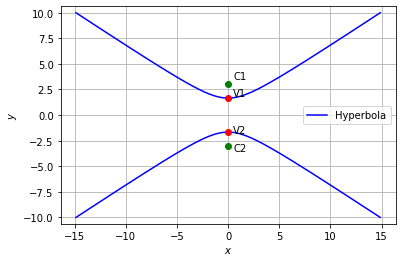
\includegraphics[width=\columnwidth]{hyperbolafig.png}
\label{fig:hyperbola}
\caption{Plot of Hyperbola}
\end{figure}
\end{document}